\section{TESTING - ignore}

\begin{figure}[h]
\begin{center}
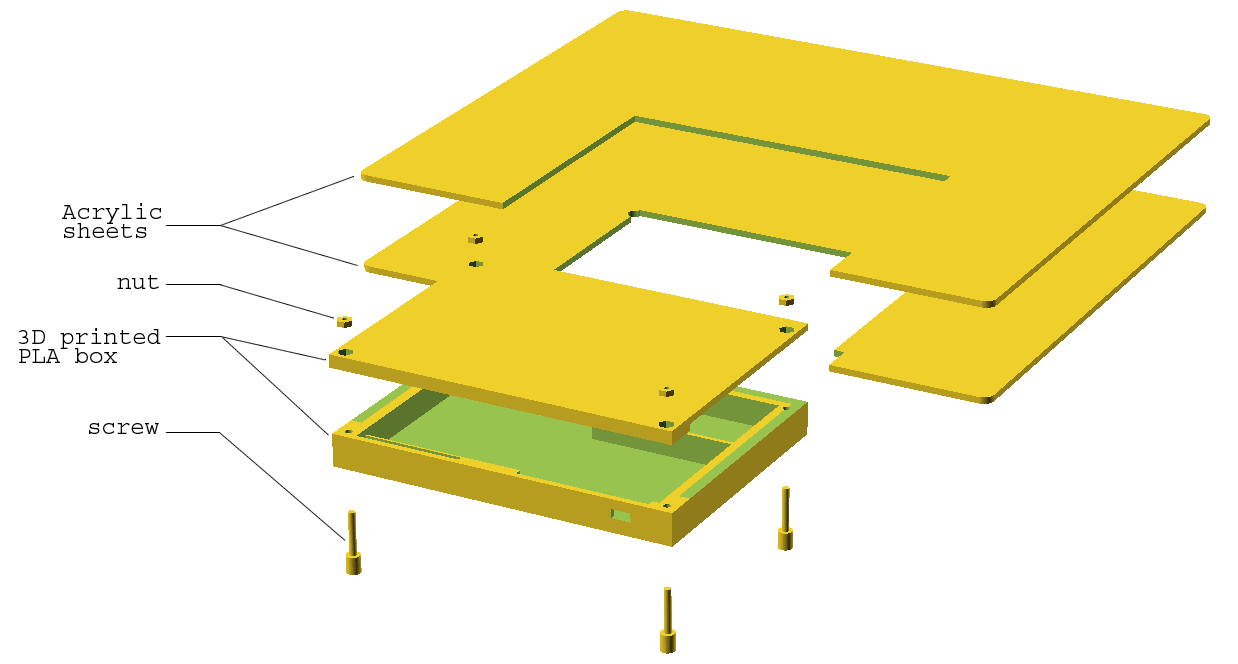
\includegraphics[scale=0.5]{figures/explode.png}
\caption{\small {\it {This is a description}}} \label{fig:explode}
\end{center}
\end{figure}


\begin{figure}[h]
\begin{minipage}[b]{7.5cm}
\centering
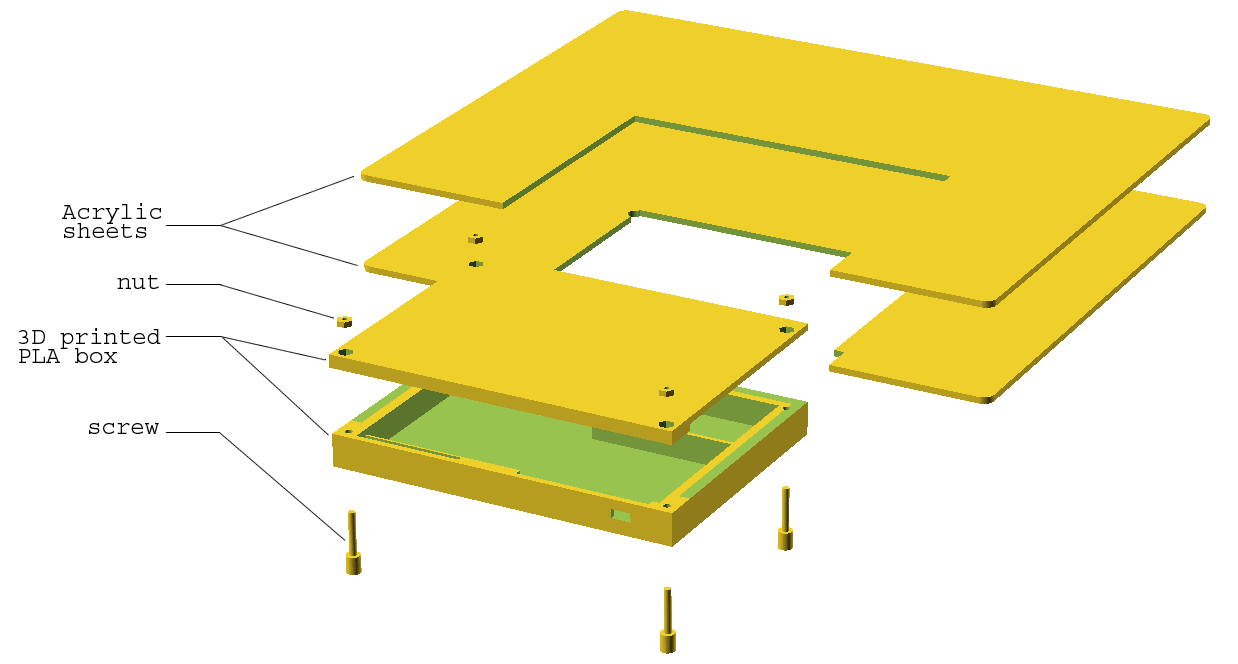
\includegraphics[scale=0.20]{figures/explode.png}
\caption{\small {\it {This is a description}}} \label{fig:testfig1}
\end{minipage}
\hspace{0.5cm}
\begin{minipage}[b]{7.5cm}
\centering
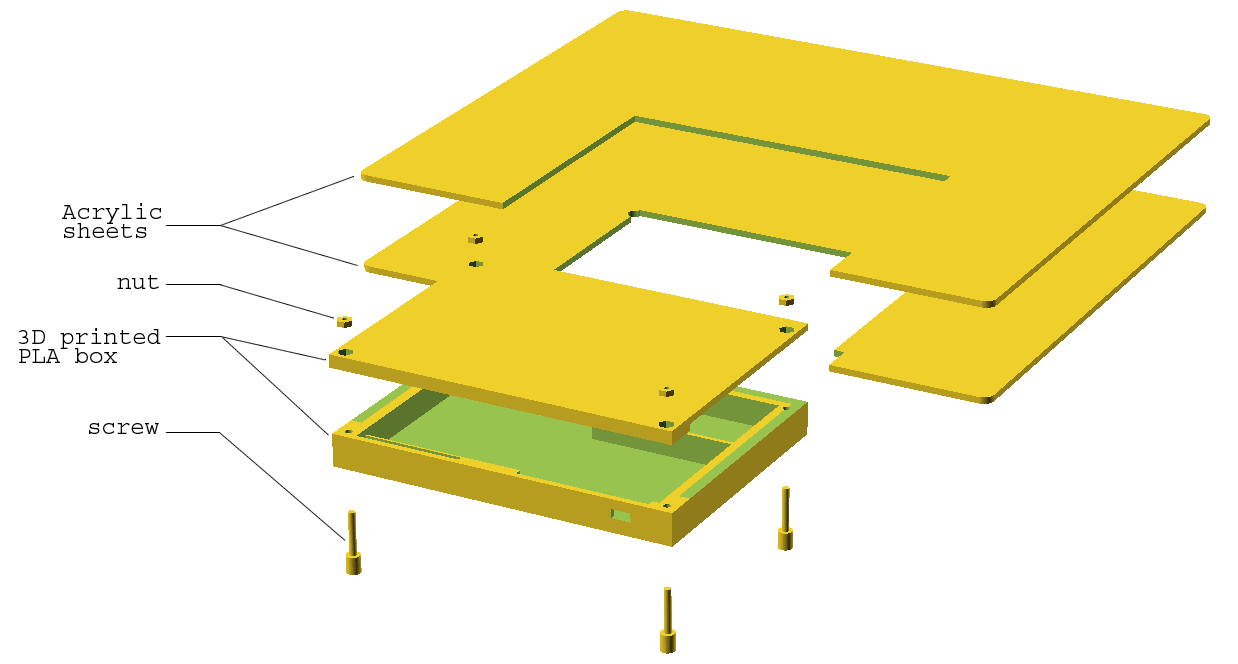
\includegraphics[scale=0.20]{figures/explode.png}
\caption{\small {\it {This is a description}}} \label{fig:testfig2}
\end{minipage}
\end{figure}


\begin{itemize} \itemsep0em
  \item The individual entries are indicated with a black dot, a so-called bullet.
  \item The text in the entries may be of any length.
\end{itemize}
